

\section{超电势}


某一电流密度下,实际发生电解的电极电势$\phi$和可逆电极$\phi_0$之间的差距称为超电势。

\subsection{极化曲线}


在给定电流$i$下,电池或电解池中阴极和阳极的实际电极电势的值称为极化曲线。总体上看由于极化的存在不利于能量的利用。

\begin{figure}[h]
    \centering
    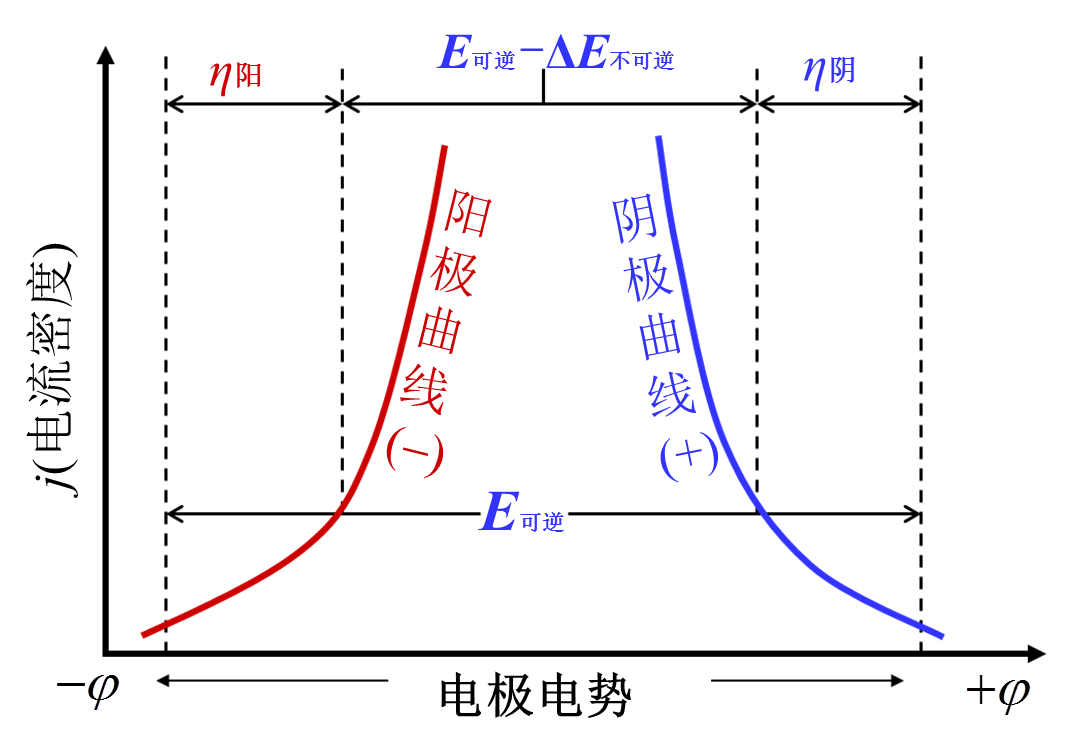
\includegraphics[width=0.7\textwidth]{battery_dmii.png}
    \caption{电池的极化曲线}
    \label{fig:battery_dmii}
\end{figure}

\begin{figure}[h]
    \centering
    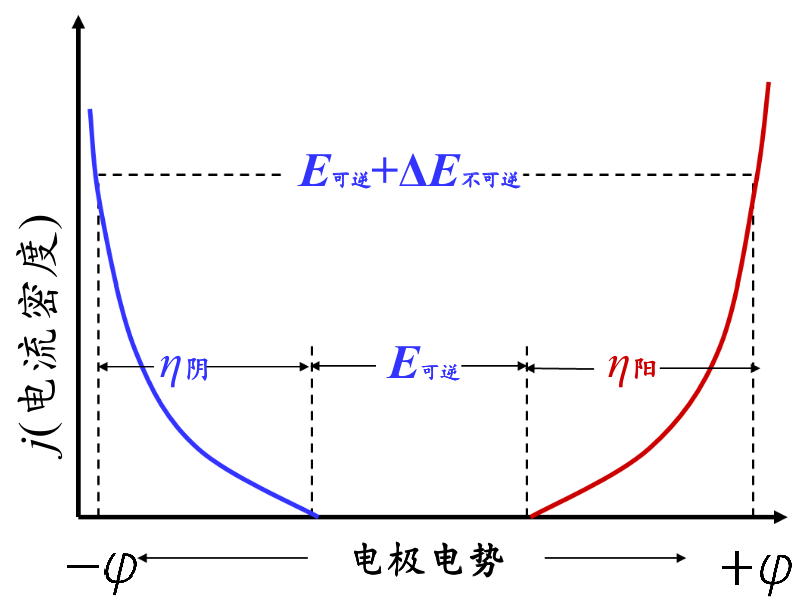
\includegraphics[width=0.7\textwidth]{cell_dmjpii.png}
    \caption{电解池的极化曲线}
    \label{fig:cell_dmjpii}
\end{figure}




\subsection{氢超电势}

电解质溶液通常用水作溶剂,在电解过程中,$\ce{H+}$在阴极会与金属离子竞争还原。
利用氢在电极上的超电势,可以使比氢活泼的金
属先在阴极析出,这在电镀工业上是很重要的。
例如,只有控制溶液的 pH ,利用氢气的析出有
超电势,才使得镀 Zn , Sn , Ni , Cr 等工艺成为现

Tafel, et al. (2007) 提出了一种新的超电势模型,其中氢超电势为

\begin{equation*}
    \eta = a + b \ln \frac{j}{[j]}
\end{equation*}

